\chapter{Introduction}
\thispagestyle{empty}
The complexity of the
nuclear many-body problem has made nuclear physics a field driven
by discoveries of outstanding phenomena. Tanihata's discovery in 1985 
\cite{isao} of vastly spatially
extended nuclei ($^{6,8}$He; $^{11}$Li; $^{11}$Be) at the neutron
dripline, 
triggered an interest in the study of weakly bound
and resonance phenomena in few-body systems.
With access to secondary
exotic nuclear beams, the edges of the nuclear landscape itself
are being explored, {\em i.e.} the very limits of nuclear
existence. At these limits, the so-called neutron (proton) {\em
driplines}, additional neutrons(protons) literally drip out of the
nucleus.  Nuclei far from stability
allow us to amplify and isolate particular aspects of the nuclear
interaction and dynamics. Using what we learn from these nuclei we
can then return to the nuclei of the world around us and
understand them far better than ever before. Progress in nuclear
structure is made at the various levels where one attempts to
understand nuclear phenomena; (i) Experimental data and
phenomenology, (ii) `Local models' (effective models with few
emergent degrees of freedom),
 (iii) `Global nuclear models',
(iv) Ab initio NN-interaction based procedures, (v) QCD.
There is an overall effort to explain higher levels in terms of
lower ones, but a more reductionist ``deductive approach'' is
likely to have as precursor an approach which tries to isolate and
understand the characteristic degrees of freedom. 

\section{Few-body aspects of dripline nuclei.}
 Nuclei along the dripline with 
an extreme dilute neutron skin have been labeled \emph{halo nuclei}. 
Understanding the mechanisms underlying the formation of such nuclei 
has been a theoretical challenge, especially two-neutron 
Borromean\footnote{ The three Borromean rings, the heraldic symbol of
the Italian Borromeo family, are interlocked in such a way that if
any of them were removed, the other two would also fall apart. The
three interwined Borromean rings are now widely used as the logo
of the halo field.} halos such as $^{6}$He and
$^{11}$Li. The Borromean nuclei display extreme clusterization into an
ordinary core nucleus and veil of halo nucleons -- forming
exceptionally dilute neutron matter. This clusterization  
has motivated few-body approaches such as the hyperspherical harmonic method 
and momentum space Faddeev equations,
to these nuclei \cite{zhuk}. Borromean nuclei such as $^{6}$He and $^{11}$Li 
has been especially suitable for few-body models, they are
characterized by pairwise constituents with no bound states but
modelled as a three-body system they achieve binding.
The extreme size of these dilute neutron excessive 
nuclei is mainly caused by the outermost neutrons being very loosely bound or
even unbound, causing a large tail in their wave functions.  
%\begin{wrapfigure}{r}[0pt]{5.5cm}
\begin{figure}[tb]
%\begin{center}
%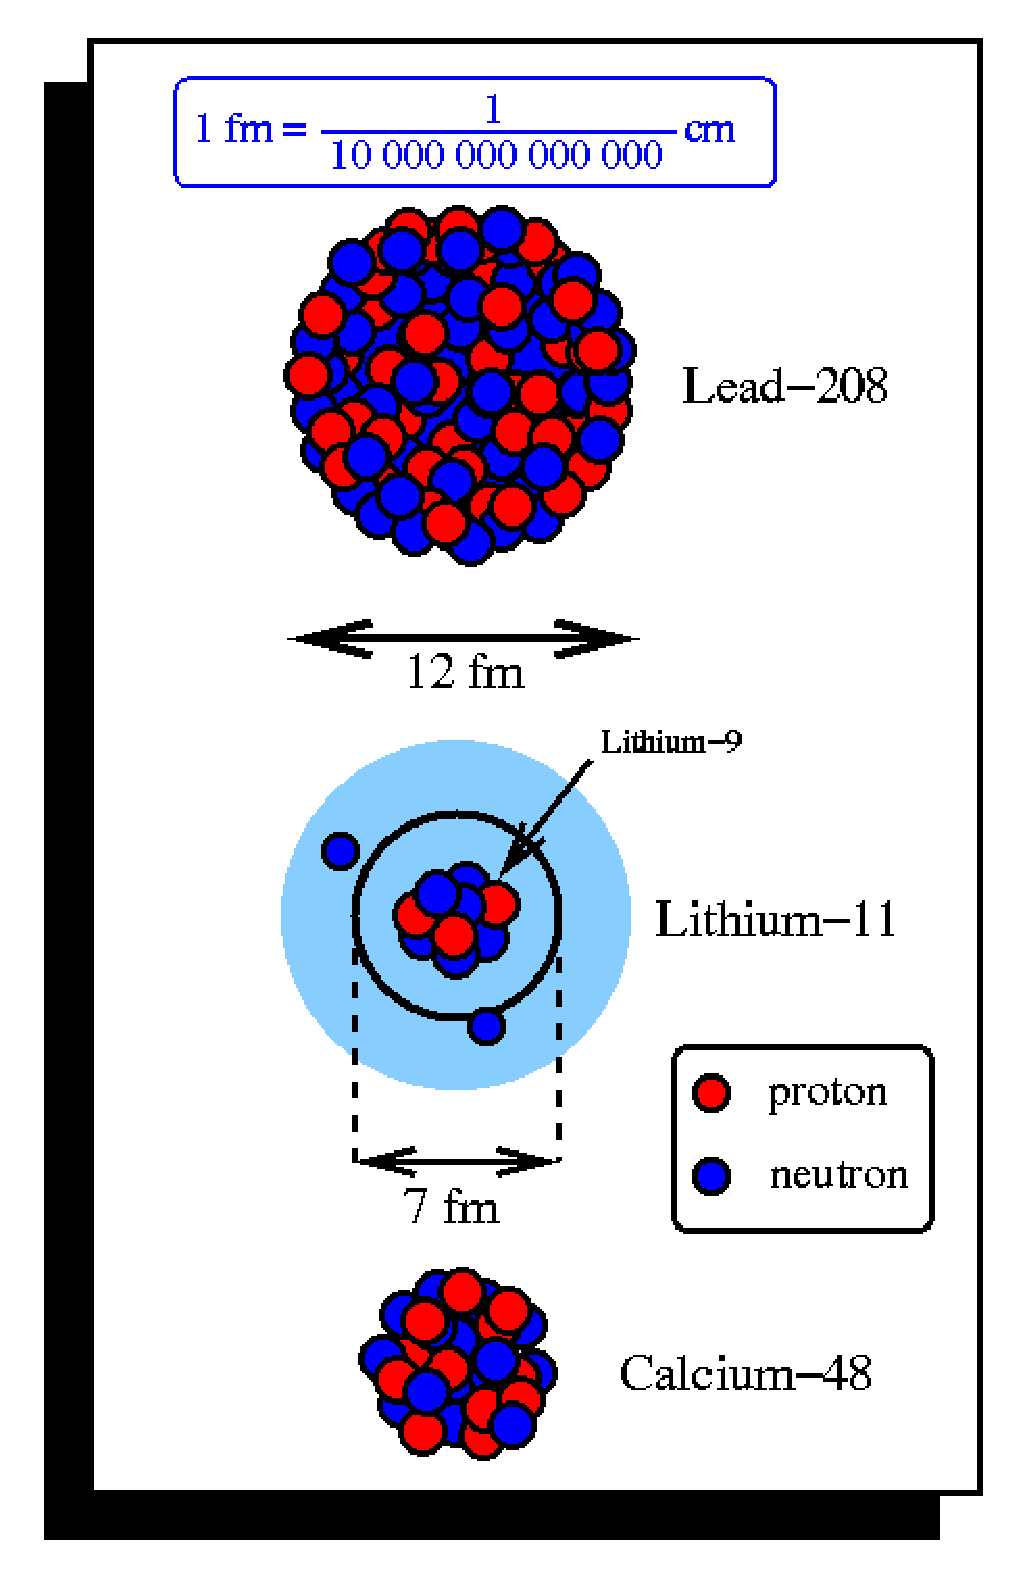
\includegraphics[scale=0.33]{lisize.eps}
%\end{center}
\centerline{\psfig{figure=figures/lisize.eps,width=8cm}}
\vspace{3mm}
\caption{The matter size of $^{11}$Li is compared to
that of $^{48}$Ca and $^{208}$Pb \label{Size} }
%\end{wrapfigure}
\end{figure}
Figure~\ref{Size} shows the spatial extension of the Borromean nuclei 
$^{11}$Li in comparison with the nuclei $^{48}$Ca and $^{208}$Pb. The spatial
extension is huge, the rms matter radius of $^{11}$Li is as large
as that of $^{48}$Ca, and the radius of the halo neutrons is as large
as for the outermost neutrons in $^{208}$Pb. 
To understand theoretically this abnormal feature of dripline nuclei 
has been a challenge over the years.


Borromean nuclei along the dripline have the property of being 
bound in their ground state. 
The ground-state properties of the Borromean nuclei $^{6}$He has been 
well understood in terms of few-body modelling \cite{zhuk}. The 
$\alpha $ core of $^6$He is stable and well bound, and it 
may be frozen in its ground state.
The relevant degrees of freedom are then described by the two halo neutrons 
relative to the core. 
In three-body models of halo nuclei such as $^6$He, Pauli blocking
is needed to remove components of the halo wave function that
would disappear under full antisymmetrization. This, and also
other aspects of the composite nature of the clusters make the
challenge somewhat different from that of three-nucleon systems.

However, most nuclei along the dripline
exhibit an unstable character, in that their ground state is embedded
in the continuum, in the form of a resonance. The hadronic stability 
of Borromean nuclei is mainly due to strong pairing effects between the 
outermost neutrons. Figure~\ref{Map} gives the hadronic
stability of various isotope chains, and it is seen that
while $^5$He is unbound $^6$He is bound, $^7$He is unbound but
$^8$He is again bound. A recent review \cite{jonson} looks at
all the dripline nuclei.
\begin{figure}[tb]
%\begin{center}
%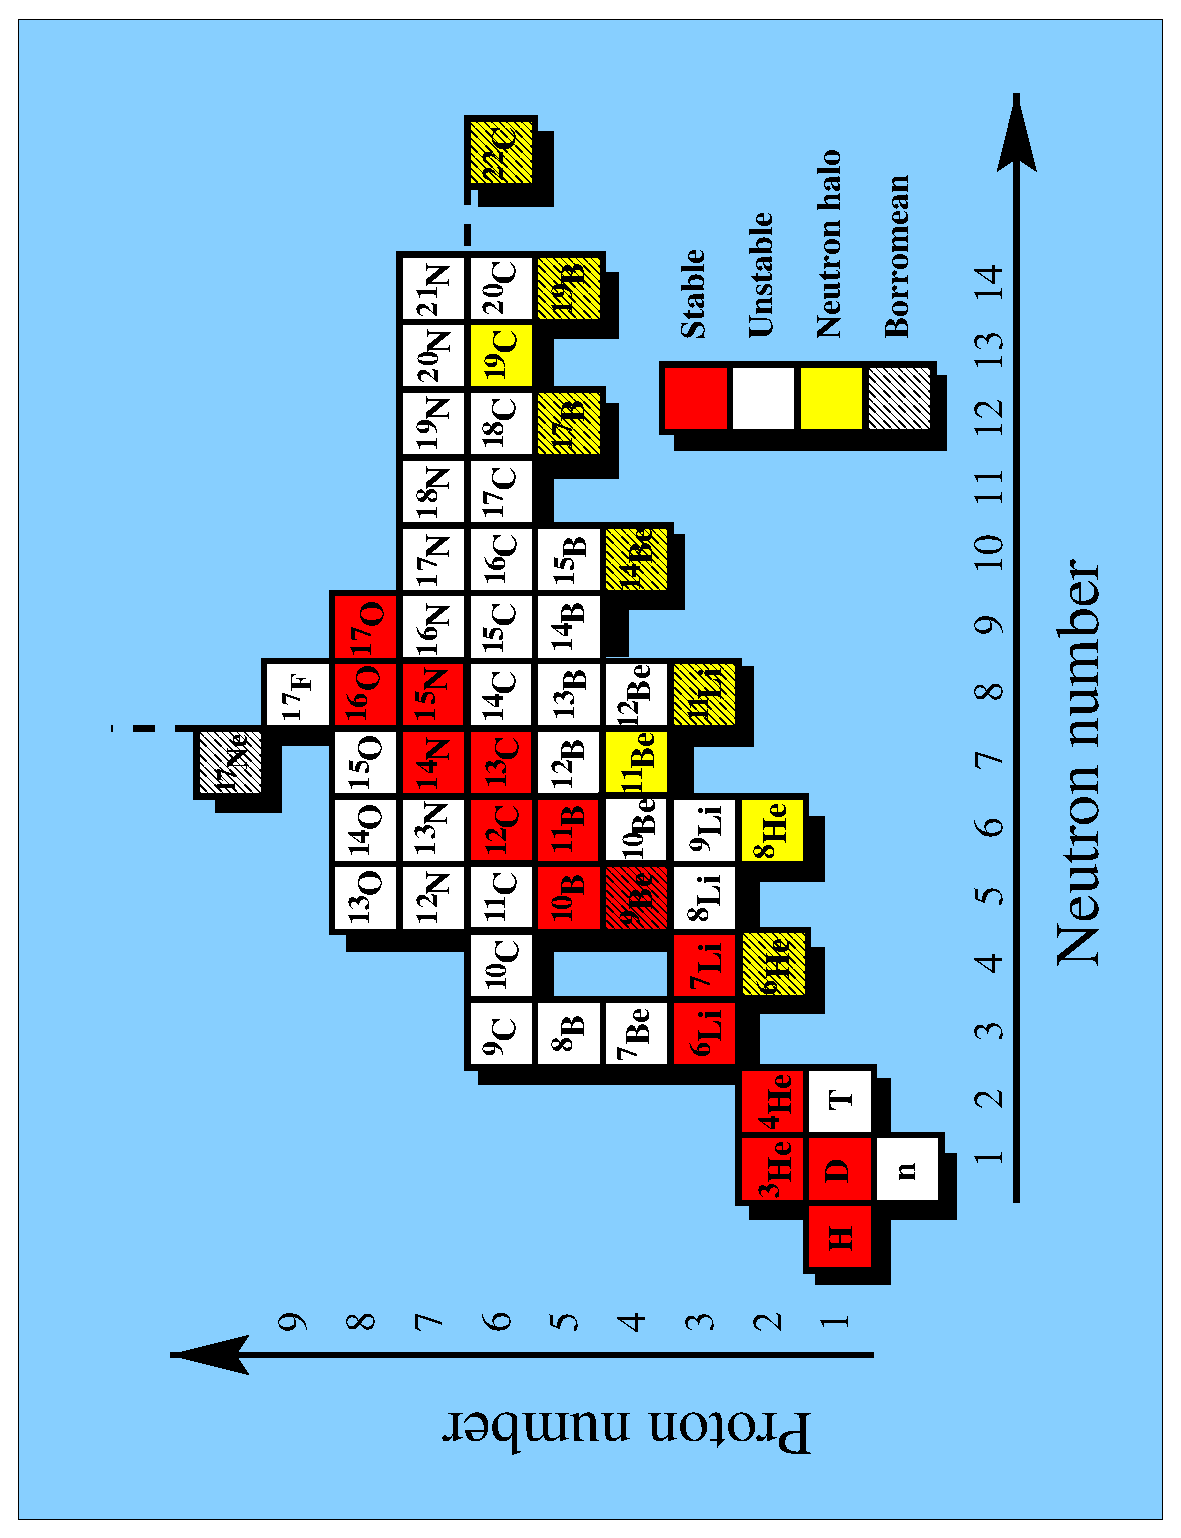
\includegraphics[scale=0.4,angle=270]{segre.eps}
%\end{center}
\centerline{\psfig{figure=figures/segre.eps,width=8cm,angle=270}}
\vspace{3mm}
\caption{The nuclear chart exhibits the stability of
Borromean nuclei among different isotope chains \label{Map}}
\end{figure}
Dripline physics, which involves nuclei  with one or a few weakly bound 
states, is physics of threshold phenomena where structure and
reaction theory merge. Hence the development of  methods for dealing with 
resonance and other continuum phenomena in such nuclei is of great importance.

\section{Resonances in quantum mechanical few-body systems.} 
The characteristic feauture of exotic states embedded in 
the continuum is that they only exist for a limited time, 
before they fall apart into their decay products. Such states are labeled quasi-stationary 
or resonant states. In a two-body picture, they may understood as states trapped inside 
the centrifugal barrier for limited time, before they tunnel through the barrier and decay.
Such resonant structures are often called \emph{shape resonances}, see figure~\ref{fig:pot_barrier}.
\begin{figure}[hbtp]
\begin{center}
\resizebox{10cm}{8cm}{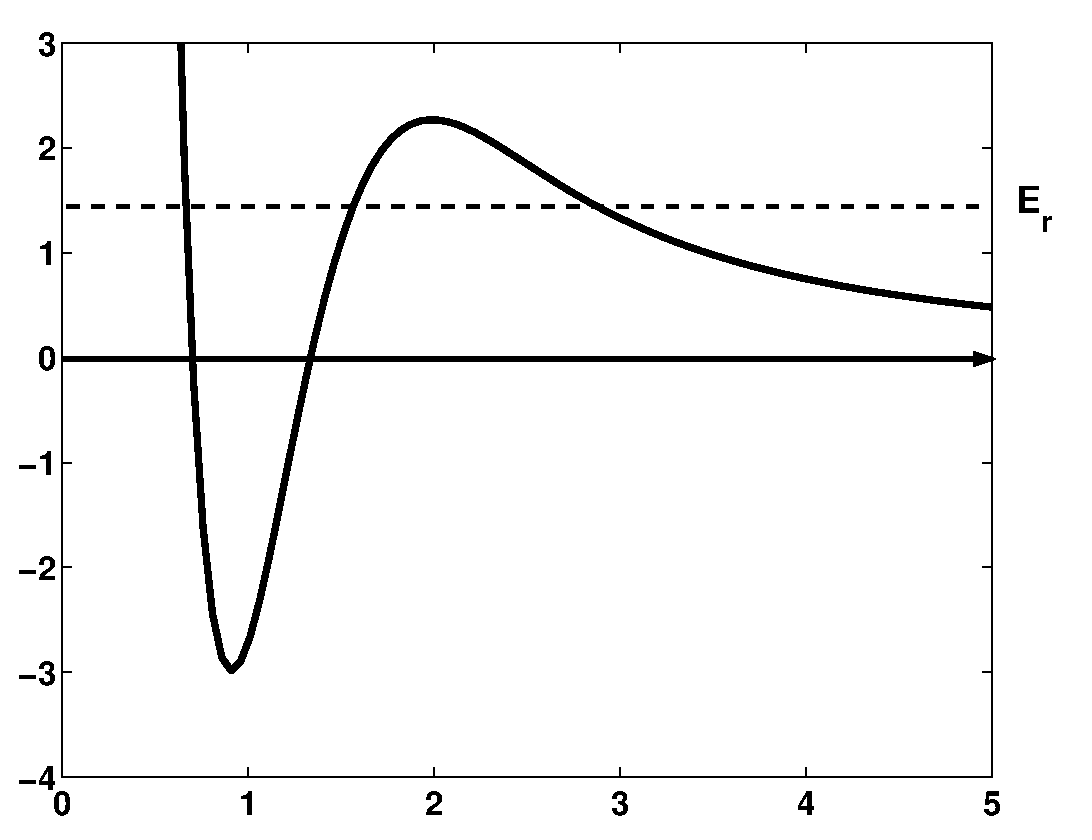
\epsfig{file=figures/pot_barrier.eps}}
\end{center}
\caption{Confining potential in which a resonant state at real energy $\mathrm{E_R}$ is formed. }
\label{fig:pot_barrier} 
\end{figure}
Considering the time dependent wave function, which satisfies the Schr\" odinger equation 
for a complex energy $z = E_R - i\Gamma /2$,
\[ 
\Psi({\bf r},t) = \Phi({\bf r})exp( -i { z\over \hbar} t),
\]
it is seen that the probability density at a point ${\bf r}$,
\[  
\vert \Psi({\bf r},t)\vert^2 = \vert \Phi({\bf r})\vert^2 exp( -i { \Gamma\over \hbar} t),
\]
decreases exponentially with time only for $ \Gamma > 0$. As already pointed out by Gamow in 1928 
in his work on radioactive decay \cite{gamow}, this wave function is the only one 
appropriate for description of resonances or quasi-stationary states. Resonances 
are observed in experiments as enhancements in the cross section when plotted
as a function of energy. In the case of isolated resonances, where the distance in energy
between the resonances exceeds their widths, and the resonaces are far from 
decay thresholds, the total cross section over the resonance peak may be parametrised 
by the Breit-Wigner formula \cite{wigner},
\[
\sigma \propto {{1\over4}\Gamma^2\over (E-E_R)^2 + {1\over 4}\Gamma^2} 
\]
A detailed analysis of such data often reveals that 
this enhancement is due to one specific partial wave. To that extent, resonances have a 
definite set of quantum numbers just like bound states, the only differences being
the fact that these states have a definite lifetime and thus correspond to 
complex energy eigenstates. Standard quantum mechanics is formulated for
Hermitian operators. This raises the question of how a Hermitian Hamiltonian 
could give rise to a complex eigenvalue and whether such states should be 
included in our Hilbert space? 

How to actually solve for single particle resonances has been a separate study 
in many different areas of quantum physics over the years.  
The specialization trend within all disciplines of 
applied quantum physics makes it almost impossible to understand 
questions and problems raised within the different branches of quantum 
physics, on the other hand a methodological unification has taken 
place in many areas. The theory of resonances is such an example.
The theory underlying the formation and decay of 
long lived states in molecules, atoms, nuclei, and condensed matter is
from a quantum mechanical viewpoint  methodologically basically the same. 
By acknowledging this, it is possible to obtain new perspectives in 
various fields by  adopting methods originally developed in
different fields of physics 
A variety of methods has been developed for understanding the basic 
mechanisms of formation of resonant states and processes taking place in the continuum.
They are described in text books such as \cite{newton, kukulin, sitenko, zeldovich}.
All the methods have in common that they originate from standard scattering theory,
and are based on the method of analytical continuation. The relevant equations are 
analytically continued from the physical energy sheet through the 
unitarity cuts onto the second energy sheet of the complex energy 
plane, where resonances may be located. 

One of the more popular methods 
during the last decades has been the complex scaling method, originally 
formulated by Aguilar, Balslev and Combes in the early 70's \cite{abc,abc1},
and developed to examine the spectrum of the Green's function on the second energy sheet. 
Later this method has been adapted in other fields
such as atomic and molecular fields to the study of resonances by complex scaling. 
In the context of complex coordinate scaling applied to quantum chemistry,
Moiseyev \cite{nimrod1,nimrod2,nimrod} developed a generalized complex variational 
principle for resonant states.
During the last decade the complex coordinate method has also been applied in nuclear physics, 
as interest in loosely bound nuclear halo systems has grown, see for 
example \cite{csoto, myo, garrido, imante} for an application to the resonant 
states of Borromean halo nuclei.
 
More recently a method based on exact differential equations for functions
closely related to the Jost functions has been developed \cite{sofianos1,sofianos2}. The
method exploits the idea of complex rotation of the coordinates, but differs from 
the traditionally used complex scaling methods using expansions and variational 
principles. The Jost function at a complex energy is obtained directly from exact equations,
and resonances are associated with zeros of the Jost function on the second energy sheet. 

Another popular approach is method based on
analytic continuation in the coupling constant (ACCC) \cite{kukulin,aoyama}.  The ACCC method
uses analytic continuation in the coupling strength of the potential instead
of the usual continuation in energy. All these methods are usually formulated in 
coordinate represenation. 

One of the disadvantages
of the coordinate space approach is that the boundary conditions have to be 
built into the equations, and convergence may be slow if the basis does not 
mirror the physical outgoing boundary conditions well. 
Instead, it is possible to represent the Schr\"odinger equation 
in momentum representation, invoking the Fourier transform. One 
of the most obvious advantages of this, is that the boundary conditions for 
bound and resonant states are automatically built into the transformed integral equations.
Diagonalizing, using a plane wave basis is very accurate \cite{hagen}, since the 
convergence is only governed by the number of integration points.

As shown by Afnan \cite{afnan1} a rotation of the integration contour in the 
lower half complex $k$-plane is equivalent to the complex coordinate rotation
method, and in this respect the coordinate and momentum space versions are complementary.
It should be mentioned that  
the contour deformation method (CDM) formulated \emph{in momentum space} is not new
in nuclear physics. It was studied and applied in the 1960`s  and 1970`s,  
see for example \cite{brayshaw,nuttal,stelbovics,glockle}, especially in the field of 
three-body systems. Most of these references
applied a \emph{contour rotation} in momentum space. By restricting 
oneself to a rotated contour certain limitations and restrictions however appear in the
equations, determined by the analytical structure of the integral kernels and potentials. 
In \cite{glockle} a more sophisticated choice of contour, 
based on rotation and translation, 
was applied to the three-nucleon momentum space Faddeev equation for a separable Yamaguchi interaction.
This choice of contour made it possible to avoid the logarithmic singularities of the Faddeev kernel
and hence allowed for a continuation in energy to the non-physical energy sheet. 
The method has recently been revived to study anti-bound and resonant 
states in subatomic physics \cite{hagen}, where a general contour was considered.

The question now arises, whether resonant states can be made part
of a complete set of states, appropriate for eigenfunction expansions. 
In the late 60's Berggren proved that for a finite range potential, 
a finite set of bound and resonant states together with a set of 
non-resonant continuum states form a complete set \cite{berggren}
of bi-orthogonal functions. 
\begin{equation}
{\bf 1} = \sum _{n}\vert\psi_{nl}\rangle\langle\psi_{nl}\vert + 
\int_{L^+} dk k^2\vert\psi_{l}(k)\rangle\langle\psi_{l}(k)\vert,   
\label{eq:berggren1}
\end{equation}
this representation has later become known as the \emph{Berggren basis}.
The non-resonant continuum integral is defined along a contour in the 
in the fourth quadrant of the complex $k$-plane, and the discrete sum is over 
both bound and resonant states. 

In this representation the usual inner-product is no longer Hermitian. 
The resonant states are not normalizable in the usual sense, as they 
oscillate and diverge exponentially along the real axis. 
As first shown by Zel'dovich \cite{zeldovich}, the inner product of
a resonant state together with its complex conjugate, may be given a definite 
value by some reguarlization procedure. 
Expanding the scattering and reaction amplitudes in this basis, makes
it possible to separate the resonance behaviour from the smooth non-resonant 
background in the scattering amplitudes. This is motivated by the 
fact that the most interesting phenomena taking place in the continuum 
are the resonance phenomena. 


\section{Modern \emph{Ab initio} approaches to nuclear structure.}
In physics one often attacks a specific problem within a reductionist way of thinking. 
That is, the phenomena of the whole system 
should be described in terms of the theories and laws of the parts of the system. 

In nuclear physics one would ideally like to start from nucleon degrees of freedom.
The dominant philosophy within the nuclear theory community is 
that the nucleus (at low energies) as a whole  may be fully described in terms of the 
the interactions between these constituents.
Building up the nucleus from these basic constituents and their mutual interactions, 
the quantum mechanical description of the many-body system however becomes extremely 
complex and hard to tackle as the number of nucleons increases. 

In the history of nuclear structure the shell model has been very
successful in describing properties of nuclei near the valley of stability.
The traditional shell model has usually been formulated in a harmonic oscillator 
representation, this is based on the assumption that 
the single particle motion within the nucleus is well described by harmonic oscillator orbitals.
This is certainly true for well bound nuclei where the tail of the single particle
wave functions fall of rapidly.
The harmonic oscillator wave functions are also favourable as
they are given in terms of well known mathematical functions. However, the possibly most attractive aspect is
that the Hamiltonian describing the motion of two particles in a harmonic oscillator potential may 
be written in separable form in both relative and center-of-mass coordinates and 
shell model coordinates. This is extremely favourable since the 
effective interaction between the nucleons are given in relative coordinates.

The shell model approaches to nuclear structure are usually not 
truely reductionistic. For heavier nuclei the number of degrees of freedom becomes 
too large to handle with modern computers. Therefore it has been customary 
to define an inert core of the nucleus which sets up a mean-field in which 
the valence nucleons move. Thus the nucleus $^{18}$O may be modelled 
with two valence nucleons moving in the $s-d$ shell with respect 
to the closed shell nucleus $^{16}$O acting as an inert core. 
As the number of valence particles grows the number of nucleon configurations 
within a valence space becomes larger and larger, making it diffucult 
to handle numerically. 
Nevertheless, in the last decade one has experienced an extreme 
development of computational power, making it possible to extend the shell model
into regions previously inaccessible. 

The growth of computational power has also sparkled a belief 
in \emph{ab initio} calculations of nuclei, taking into account all 
degrees of freedom. The most ambitious of these `reductionist' attempts are Green's
Function Monte Carlo (GFMC) calculations \cite{pieper1,pieper2,pieper3,pieper4,pieper5,pieper6,pieper7}, 
extending previous variational Monte Carlo (VMC). According to the authors
these are the first microscopic calculations that directly
produce nuclear shell structure from realistic interactions that
fit NN scattering data. Another line of approach are the
large-basis no-core shell-model (NCSM) calculations of Barrett's
group \cite{bruce1,bruce2,bruce3,bruce4}, where the shell model is combined with
microscopic effective interactions derived from modern
nucleon-nucleon potentials. 

The exponential growth of the configuration space as the number of
active particles increases makes it extremely difficult to reach 
into the range of medium size nuclei, within these \emph{ab intio} 
formalisms. The cost of matrix diagonalization increases as the third power
of the number of basis states, and the memory required to store the 
Hamiltonian matrix increases as the square of the number of basis states.
The practitioners have, however, already had success with their
pioneering attempts. So far converged results for nuclei with up to $A = 12$ 
active particles have been reported. Further, GFMC and NCSM calculations 
for A=6 do produce an alpha-like core object, and two alpha-particles for $^8$Be,
both promising features.

Another \emph{ab initio}�
approach which recently has proved promising in the 
medium size region of the nuclear chart, is the Coupled-Cluster method.  
The Coupled-Cluster method originated in nuclear physics in the 60's 
\cite{cc4,cc5}, but has since that time only appeared sporadic within 
nuclear physics. On the other hand Coupled-Cluster theory has 
been extensively used, and with great success, 
in quantum chemistry over the years \cite{cc6,cc7}. 
Basically the Coupled-Cluster method  is based on an 
exponential ansatz for describing correlations within a nucleus. 
\[ 
\Psi_{CC} = exp(\hat{T})\Psi_0, \:\: \hat{T}�= \hat{T_1} + \hat{T_2} + \hat{T_3} +...,
\] 
where $\hat{T}_n$ are linear combinations of all $n$-type excitations. 
Including only single and double excitations (CCSD), the computational cost 
scales as $ N^7$�where $N$ is the size of the system. Instead of direct matrix
diagonalization, a non-linear set of equations is solved iteratively. 
Very recently \cite{cc1,cc2,cc3}, converged Coupled-Cluster 
results for the ground- and first excited state of $^{16}$O have been reported, using 
modern nucleon-nucleon interactions derived from effective field-theory.

\section{Exotic many-body states embedded in a continuum.}
All of the above mentioned many-body approaches have been formulated using 
a harmonic oscillator basis describing single particle motion. 
Adopting a harmonic oscillator picture, one assumes from the very 
start that the interacting nucleons are isolated from an external environment
of positive scattering states. The tremendous success of the multi-configurational 
shell model over the second part of the last century, in describing properties of nuclei
where continuum aspects are more or less absent, has given little focus on mechanisms 
involved in the formation and decay of nuclei far away from the valley of $beta$-stability. 
However, approacing the drip-lines
new aspects and properties of nuclei emerge, such as the instability of decay, enormous size 
of halo nuclei and the melt down of shell structures and new shell closures. 

To bridge the gap between reaction and structure theory,
microscopical shell model calculations using a Berggren representation for the
single particle states were proposed some years ago \cite{lind,liotta}. 
The proximity of the scattering continuum in weakly bound and unbound nuclei,
implies that these nuclei cannot be properly described without taking into 
account the coupling between discrete states and   the 
positive energy continuum. In other words, a proper description of loosely bound 
nuclei should take into account the coupling of the internal with the external 
environment, which has been totally neglected in classic shell model approaches.
The coupling of the 'external' continuum of positive energy states, with the 'internal' 
nuclear states has for a long time been basic ingredient in nuclear reaction theory. 
Feshbach was the first to formulate a unified description of direct and 
compound nuclear reactions within the projection operator method \cite{feshbach1,feshbach2}. �
He showed that the coupling of the internal with the external environments could 
give rise to compound nuclear states, such as 
multi-channel resonances. As he was the first to 
formulate a general theory of such states, they became known as Feshbach resonances. 
Also in atomic physics Feshbach resonances
are of great importance. In the early 60's, at the same time of Feshbach's work, Fano \cite{fano} 
discussed how the mixing of a configuration 
belonging to a discrete spectrum with configurations belonging to a continuous spectrum
gives rise to the phenomena of \emph{autoionization}, which is considered a multi-channel 
resonance or in other words a Feshbach resonance.

Entering the realm of weakly bound nuclei, it becomes evident that the 
standard separation of nuclear structure and nuclear reaction methods has
to be abdoned. A merging of the two fields, where many-body methods from the 
structure community are united with reaction theory, where the importance of the
continuum has been studied over several years, seems to be a fruitful way of approach.
Treating the continuum aspects properly within existing many-body theories, 
is however much more difficult than when dealing with well bound nuclei.
Existing many-body structure approaches have to be reformulated and developed further since 
the harmonic oscillator representation has to be abdoned. 
All the nice 
mathematical properties of the harmonic oscillator basis are non-existent 
in all other single particle representations, e.g. the Woods-Saxon basis. 

Having determined a single particle basis consisting of bound, resonant and 
non-resonant continuum states, it is natural to again focus on the 
application of this basis in nuclear structure calculations of weakly bound and/or 
unbound nuclei. Ideally one would like an \emph{ab intio} description
of these nuclei, taking into account all relevant degrees of freedom. In the 
hyperspherical description of three-body Borromean and halo nuclei, 
the problem of treating core excitations and the anti-symmetrization between core and valence 
nucleons has not fully been solved. Treating such nuclei microscopically, a reformulation 
of the shell model using a single particle basis of bound, resonant and scattering states 
may appear to be the most straightforward method. 
The recently developed Shell Model Embedded in the Continuum (SMEC), see e.g.  
Refs.~\cite{csm1,csm2,csm3,vz2003}, offers such a possibility. 
SMEC is closely related to the Feshbach projection operator technique. 
In SMEC the bound,resonant and scattering states are treated on equal footing,
by introducing two subspaces and taking their coupling into account.
However, most SMEC calculations have not taken into account coupling with decay channels  
containing more than one nucleon. 

Restricting the theory to only one-nucleon 
decay channels, limits the applicability of SMEC along the drip-lines. Borromean 
nuclei for which the $A$�and $A-2$ nuclei are particle stable, while the nuclei $A-1$ are not, 
requires a theoretical description which takes into account decay channels involving all valence 
nucleons. That is, all many body configurations involving bound and scattering states should 
be considered. 
The newly developed Gamow shell model is devoted to such an approach, see for example 
Refs.~\cite{michel1,michel2,michel3,liotta,betan,witek1,witek2,roberto,betan2,hagen}.
The Gamow shell model starts with the Berggren representation (\ref{eq:berggren1}) for single particle states. 
A complete many-body Berggren basis may then be constructed from the 
discretized single-particle Berggren orbitals
\[ 
\sum_n \vert \Psi_n\rangle \langle \tilde{\Psi}_n\vert = 1,
\]
where the many body Slater determinants $\vert \Psi_n\rangle $�are constructed 
from the discrete bound, resonant and non-resonant continuum orbitals.
This is in full analogy with the standard shell model 
using a harmonic oscillator basis.  
When the exact multi-particle resonance wave function is expanded in a complete 
set of Slater determinants consisting of discretized single particle Berggren 
orbitals,  an interpretation of these exotic multi-particle structures
in terms of single particle resonances becomes possible. 

Intuitively one would expect that the 
Slater determinant built from single-particle resonances only, would be the
major component in the fully correlated many body wave function. This is certainly true
if the residual nucleon-nucleon interaction is weak compared with the 
mean-field in which the valence particles move. More interesting is the opposite
case, where the residual interaction is strong. In this case it is not 
obvious that the pure pole configurations are the most important. However, 
the Gamow shell model may provide an answer to the question of how exotic 
structures, such as multi-particle resonances, embedded in the continuum are formed.
The Gamow shell model is a promising many-body approach in the study of unstable nuclei
along the drip-lines. And it is in the unifying spirit of scientific development, in that it
reconciles the reaction and the structure part of the community. 
The Gamow shell model is in its early stages, and so there exist  a vast 
area of applications and mayor theoretical and computational challenges to be dealt with.
One of the first challenges and problems encountered in the Gamow shell model, was
the \emph{identification problem}, and first addressed in \cite{liotta, betan}.
The physical multi-particle resonances 
will in many cases be embedded in a dense distribution of continuum states, 
depending on the contour on which the continuum states are defined.  
Refs.~\cite{liotta, betan} related this \emph{identification problem} to 
the problem of choosing a contour in the complex $k$-plane which 
in the case of several valence particles selects the physical interesting
states from the dense continuum background. They found that in the two-particle
case, choosing a \emph{square-well} contour makes an identification 
of physical states based on 
inspection of the zeroth order energy surface possible. This solution is
only  applicable in the two-particle case,  already in the tree-particle case
the physical states get mixed in with the continuum states.
In Refs.~\cite{michel2,witek1,witek2} the problem of identifying multi-particle 
resonances was approached from a different angle.
The proposed algorithm is a two step procedure. In the first step 
a diagonalization within the pole space, where all particles are in 
resonant single particle orbitals, is performed. Secondly a 
diagonalization within the complete configuration space is done.
Under the assumption of weak coupling of the pole configurations
with the configurations where at least one particle moves in a continuum orbital, 
the physical states may be picked out unambiguously from the states obtained after a 
full diagonalization, using the criterion of largest overlap with the pole space.
The weak coupling limit may not always be a valid assumption, as pointed out in Ref.\cite{betan2} 
for the case of $^{11}$Li the two-particle resonances may
have a larger continuum component as compared to the pole component,
depending on the strength of the residual nucleon-nucleon interaction.
Presently one may conclude that the \emph{identification problem} has not
been solved generally, and developing an algorithm which picks out 
physical states unambiguously from the dense continuum background is still an open problem.

Another challenge for the Gamow shell model is the \emph{dimensionality problem}. As the number
of active particles moving in a valence space increases, the 
number of Slater determinants in the many-body Berggren basis increases dramatically. 
This explosion of many-body configurations is  even more severe than in the 
standard shell model approach where only bound states appear. In the Gamow shell model
one has for each partial wave a finite number of non-resonant continuum states which are absent
in the standard shell model. In solving this problem, one has to take advantage of 
effective operator and perturbation method techniques 
typically used and developed for large scale shell model 
calculations using harmonic oscillator bases. 

With further progress in computational power   
one may hope that \emph{ab intio}  calculations of light and medium 
size nuclei within the Berggren representation may become possible in the near future. 
Coupled-Cluster techniques has proven to be a promising method for 
microscopical calculations of medium size nuclei such as
$^{16}$O,
a promising way of approach would be 
to generalize the Coupled-Cluster method to complex interactions, and
at the first stage see how resonant structures are formed in light nuclei
starting from an  \emph{ab initio} approach. Another interesting application 
would be to see how single particle resonances are formed starting from 
a realistic nucleon-nucleon interaction. In conclusion, one may say that 
nuclear physicists are living in exciting times.


\section{Outline of Thesis.}
This thesis combines results which are published in 
international journals with 
results which appear only in this thesis. 
The main purpose of this thesis, may 
nevertheless be summarized in the two published papers   
{\it The contour deformation method in momentum space, 
applied to subatomic physics}  and 
{ \it Effective Interaction 
Techniques for the Gamow Shell Model}. However, since
these papers deal with topics which may be less familiar to 
the audience, this thesis aims at giving 
a more detailed and thorough discussion of the formalisms and theories
underlying this work. The outline of the thesis is the following. 

Chapter~2 gives a detailed discussion of the scattering functions
and Jost functions starting with the coordinate representation 
of the Schr\"odinger equation.  The most general distribution of 
poles of the scattering matrix is discussed, together with their 
physical interpretations. Chapter~2 also dicusses some 
typical regularization procedures for matrix elements involving 
resonant states. An outline of the proof of the general 
Berggren completeness which includes bound, anti-bound and resonant
states is given, and a discussion of the physical 
interpretation of expectation values of observable operators
involving resonant states.

Chapter~3 starts with the momentum representation of the 
Schr\"odinger equation (Section~\ref{sec:momspace}), 
and discusses how the Schr\"odinger equation 
may be analytically continued to the second energy sheet using 
the Contour Deformation Method (CDM) 
(Section~\ref{sec:analytic_continuation}).
A complete set of 
single particle states, involving all kinds of poles, 
is obtained. Chapter~3 contains several applications
which are not included in the published papers. 
Section~\ref{sec:deformed} gives an application of the CDM to the 
problem of solving for resonances in a deformed field is given 
Section~\ref{sec:optical} gives an application of CDM to 
resonances and bound states in complex absorbtive and emitting 
potentials.
Section~\ref{sec:inmedium} gives an application of CDM 
to the solution of pair instabilities of the CD-Bonn interaciton 
in a infinite nuclear medium, and discusses how 
poles on the second energy sheet may be interpreted as resonance
like states. 


Chapter~4 discusses the application of a single-particle
basis constructed by CDM may serve as a starting point
for Gamow-Shell-Model studies. Section~\ref{sec:lanczo}�
discusses how the Lanczos iteration method may be applied to 
the calculation of multi-particle resonances in the Gamow Shell
Model formulation. As numerical test study, the convergence
of the $0^+$ ground state and the $2^+$ resonance energy of 
$^6$He for each iteration is given. The results are promising for
large-scale Gamow Shell Model calculations. 
Section~\ref{sec:lee_suzuki}
gives a formal derivation of the Lee-Suzuki similarity
transformation method for complex interactions, and shows 
how a complex symmetric interaction may be obtained 
by a second similarity transformation. Section~\ref{sec:multi_reference}
discusses the use of Many-Body perturbation theory in 
Gamow-Shell-Model calculations. A derivation of the standard
Rayleig-Schr\"odinger perturbation expansion for 
a single model space state is given for the case of complex
interactions. It is shown that the standard single-reference
perturbation theory does not give satisfactory results
when treating many-body resonance perturbatively. The
Multi-Reference-Perturbation-Theory-Method (MRPTM) is
subsequently derived. This theory differs from 
standard perturbation theory, in that it is a  
one-state-at-a-time perturbation theory. Finally, 
Section~\ref{sec:effective_scheme} gives an effective
interaction scheme for the Gamow-Shell-Model 
which combines the Lee-Suzuki similarity 
transformation method with the one-state-at-a-time MRPTM. 

Chapter~5 gives a short introduction to the 
article {\it The contour deformation method 
in momentum space, applied to subatomic physics}. 

Chapter~6 gives a short introduction to the 
article { \it Effective Interaction Techniques for the Gamow Shell Model}.

In Chapter~7 conclusions of the present work, and future 
perspectives are given.  



 
 




% shell model embedded in the continuum. 






